\chapter{Results}

In this chapter I am going to illustrate the results obtained when running the algorithm. This include an evaluation of the system free energy and site overlaps. It is possible to give a quantitative description of the correctness of the solution. This will be done in the final section, introducing a RSB sensitive parameter and comparing the result obtained in \cite{bethe}, the results obtained from \cite{zullo} and ours.

\section{Evaluation of $x_{C,max}$ and $x_{s,max}$}

In order to evaluate the thermodynamic procedures, it is well known that first of all one must maximize the free energy respect to $x_s$ and $x_C$.
We will call  $x_{C,max}$ and $x_{s,max}$ the two values that determine the maximum.
A direct computation of the free energy is possible using the corollaries in appendix III. Our task is to find a maximum of $F$ inside the range
$(x_s,x_C)\app \[(0,1) \times (0,1)\]$.

I made several runs of the algorithm, varying $x_s$ and $x_C$ and evaluating the mean free energy on many iterations.
Since a previous evaluation of one step RSB $x$ has been made \cite{bethe}, finding a value for $x_{max} = 0.24 $ and an incredibly accurate estimation of the free energy, we will expect to find the two values in a region close to the couple $(x_{max} , x_{max})$.




\section{Various run methods}

Since we have more than one task to accomplish, every run of the algorithm will differ a bit from the others, depending on which is the main goal of that particular run.
In order to explain better, let us summarize each run and its goal.

\begin{enumerate}
 \item{Find the region which maximizes $F$. This can be done with low precision, just to give a hint on where to concentrate in future.}
 \item{Perform high precision runs on the region found previously. The goal is to find the correct couple $X \equiv(x_C,x_s)$ with sufficient high precision.}
 \item{Perform a number of runs with different values of $N_c$, $N_s$ and $N_h$. This will allow us to extrapolate the thermodynamic limit using an interpolation.}
 \item{Once the couple $X$ has been found, we can perform a number of simulations with parameters $X$, in order to get each observable with relatively small error}
\end{enumerate}

A first computation has been made using low values for $N_h$, $N_c$ and $N_s$. This will give us a first hint on where to find the searched maximum.

\begin{figure}[h]
	\centering
		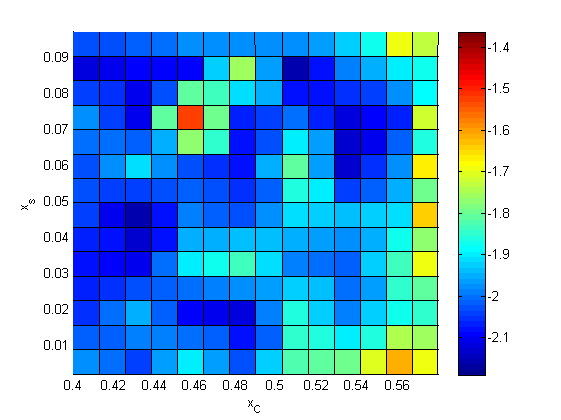
\includegraphics[scale=0.8]{img/generic_F.png}

		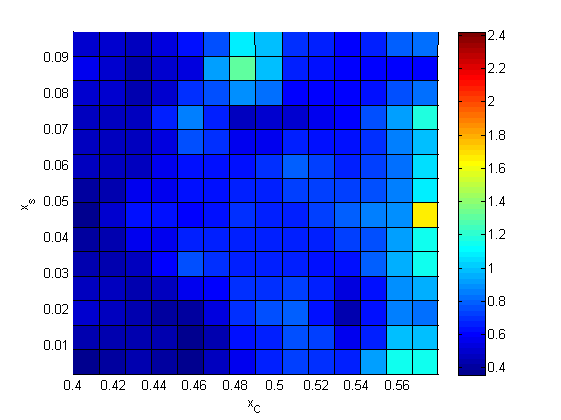
\includegraphics[scale=0.8]{img/generic_err.png}
\caption{Evaluation of F using brute force. 64 runs have been performed with low precision. }
\end{figure}

As we can see from figure, even if the free energy value is wrong we are now able to determine the correct region for our investigation.
Once the best region has been found, it is possible to enclose the search range in a neighborhood of these values.

\begin{figure}[h]
   \centering
		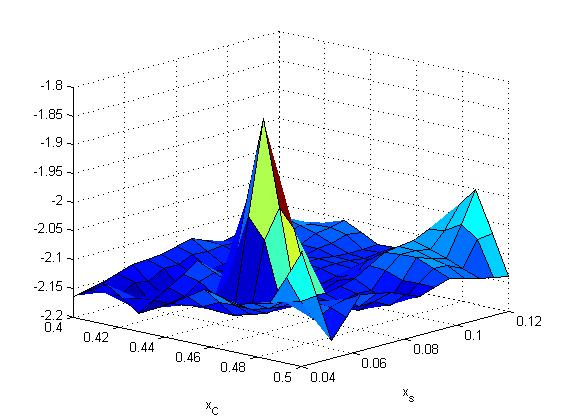
\includegraphics[scale = 0.6]{img/refined.jpg}
\caption{Evaluation of F in a smaller region}
\label{refined}
\end{figure}

From a finer computation we can see that the couple that maximizes the free energy is given by:

\begin{equation}
x_{s,max} = 0.07 \pm .01 \hspace x_{C,max} = 0.45 \pm .05
\end{equation}

Results obtained have an easy interpretation; in fact it is possible to make two interesting argumentations:

\begin{itemize}

\item{The value of both $x_C$ and $x_s$ is clearly nonzero, this
			means that replica symmetry is broken at a cluster level.
			It is now almost sure that the exact solution involves continuous RSB. Going to higher levels of RSB however would need a large computation effort.}

\item{The error in the determination of the maximum is much larger in the $x_C$ direction, evidencing the fact that the evaluation of two step RSB corrections need a greater computation effort to be
    evaluated.}
\end{itemize}

\newpage

\section{Analysis of finite-size error}

Now we evaluate the dependence of the observable averages returned by the algorithm from the sample size.
What we will do is to evaluate the average free energy of the system as a function of $N$, and then plot $F(N)$ versus $N^{-1}$. The $N\rightarrow\infty$ result is extrapolated from a polinomial fit on the obtained distribution
\begin{figure}
	\centering
		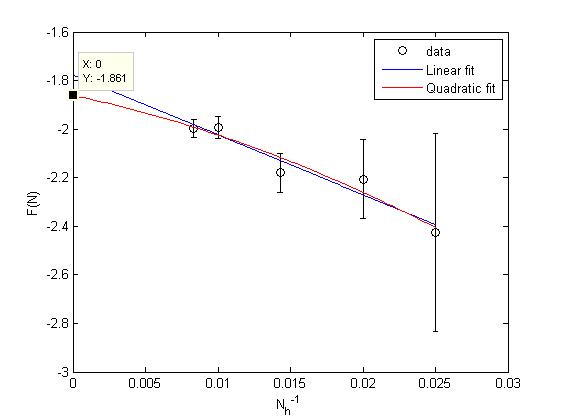
\includegraphics[scale = 0.6]{img/polyN.jpg}
		\caption{Polinomial fits of the efficiency of the results}
\end{figure}

The algorithm runs have been performed first on a domestic computer. We can see from the figure that the measurements are affected by large sistematic errors at low values of $N$. Using a domestic computer it was possible to reach values of $N$ not greater than 50.
In the figure shown above we can see that, due to limited computation capability, our algorithm cannot make a sufficienly accurate prevision in the thermodynamic region (large $N$).

It is expected that good results may be obtained with values of $N$ in the surroundings of 500. Since these numbers are out of the range of my personal computer, the simulations are currently in preparation for a run on a cluster calculator located in Sapienza University.

%We can compare the finite-size error of the two evaluation methods for the free energy $F$.
%We remark that we previously found two alternative methods for the free energy evaluation that were given by

%\begin{eqnarray}
%F &=& {K+1\over 2} F_l - K F_s \nonumber \\
%F &=& {K+1\over 2} F_{iter} - {K-1 \over 2} F_s \nonumber
%\end{eqnarray}


 %\begin{figure}
 %	\centering
 %		\includegraphics[scale = 0.6]{img/comparison.jpg}
 %		\caption{Polinomial fits of the efficiency of the results}
 %\end{figure}




\subsection{Another finite size problem}

Since the reweighing procedure only reshuffles the fields according to their free energy shifts (equation \ref{dfiter}), it is possible that, after a certain number of iterations, the population is sampled from a restricted set of clusters. By iterating again could rise the possibility of sampling the population from a single cluster. If we look equation \ref{dfiter} and try to compute $\Delta F$ using a populations where all clusters are the same, we may end having a problem in the free energy evaluation (depending on the particular type of error occurred the free energy evaluation could lead to a machine $0$ or a Nan). In order to avoid this possibility, I decided to add a
small perturbation to the evaluation of the $h_0 ^ {\alpha\gamma}$ fields. From physical argumentations \cite{vulpiani} one can deduce that the correct states distribution $Q(h)$ is left invariate under little perturbations of itself. This granted a sufficiently low reshuffling of each state distribution within each cluster. Obviously the insertion of a noise underestimates the overlaps



\section{Observables}

\subsection{Site Observables}

There are now three site overlaps that must be evaluated:
\begin{itemize}

\item{The self overlap, $q_2$, computed averaging over each state $\gamma$ and over each cluster $\alpha$}
\item{The same state overlap, $q_1$, computed averaging over each state $\gamma'$ different from $\gamma$}
\item{The interstate overlap, $q_0$, computed averaging over each cluster $\alpha'$ different from $\alpha$, and over each state $\gamma'$ different from $\gamma$}

\end{itemize}

\begin{eqnarray}
	q_2 = \sum_{\alpha, \gamma } \tanh(\beta h^{\alpha\gamma})\tanh(\beta h^{\alpha\gamma})  \\
	q_1 = \sum_{\alpha, \gamma} \sum_{\gamma' \neq \gamma } \tanh(\beta h^{\alpha\gamma})\tanh(\beta h^{\alpha\gamma'})  \\
	q_0 = \sum_{\alpha, \gamma} \sum_{\gamma' \neq \gamma, \alpha' \neq \alpha} \tanh(\beta h^{\alpha\gamma})\tanh(\beta h^{\alpha'\gamma'})  \\
\end{eqnarray}

Each of these values is then averaged over every site and every iteration.
A computation of these values near the critical point $X = (x_{s,max},x_{C,max})$ gives back these three values for the overlaps

\begin{eqnarray}
	q_2 = 0.71 \pm .005\nonumber \\
	q_1 = 0.31 \pm .03 \nonumber \\
	q_0 = 0.19 \pm .03 \nonumber \\
\end{eqnarray}

It is possible to give a quantitative evaluation of the correctness of the two-step RSB implementation. Let us define
\begin{equation}
R = \int q^4 P(q)dq - (\int q^2P(q)dq)^2
\label{erre}
\end{equation}

It is worth noting that in a RS theory $R=0$, while in \cite{bethe} the authors obtain $R = 0.047 \pm 0.002$. Simulations return a value for $R=0.056 \pm 0.001$, while the one obtained in the 2 step RSB framework can be evaluated as follows:
\begin{equation}
P(q) = p_0 \delta(q-q_0) + p_1 \delta(q-q_1) + p_2 \delta(q-q_2)
\end{equation}
where each $p_i$ is given by
\begin{eqnarray}
p_2 = (x_C) \nonumber \\
p_1 = (x_s - x_C) \nonumber \\
p_0 = (1 -  x_s)  \nonumber \\
\end{eqnarray}
A direct computation returns a value for $R =0.06$, with an high error associated:

\begin{equation}
                        R =0.06 \pm 0.02
\end{equation}

We may note that the error on the estimation of $R$ is very high. This is due to the imprecise location of $x_C$ at finite cluster size, together with a high variability of $R$ on small changes of the overlaps and the two values of the $X$ couple. Since R depends on five parameters, only a very accurate estimation of these will lead to a value

I would like to end this section with a plot of the $q(x)$ function, limited to the two step RSB framework. This has been painted using the three overlaps found previously

\begin{figure}
  \centering
  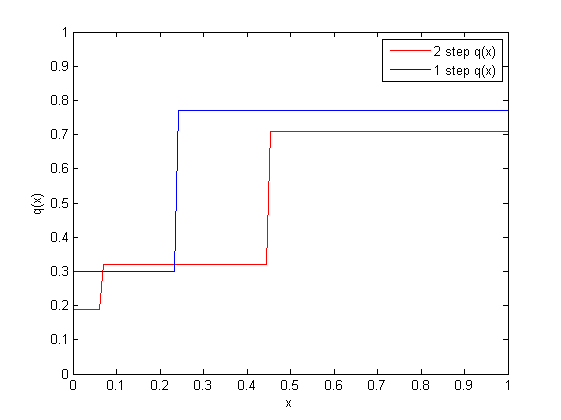
\includegraphics{img/q_function.png}
  \caption{Evaluation of R}
\end{figure}
\subsection{Link Observables}

First of all we report the evaluation of the link overlaps.

\begin{eqnarray}
	q_2^{l} = 0.73 \pm .01\nonumber \\
	q_1^{l} = 0.28 \pm .03 \nonumber \\
	q_0^{l} = 0.17 \pm .03 \nonumber \\
\end{eqnarray}

The next variable we want to compute is the internal energy of the system, given by equation

\begin{equation}
U = - \sum_{\alpha \gamma} \tanh{\beta v^{\alpha\gamma}
\end{equation}

A computation of $U$ returns a value in very good agreement with the simulations:


\begin{equation}
U = -  1.799 \pm 0.001
\end{equation}

This result needs a particular remark, since $U$ is the only observable easily computable in Monte Carlo simulations.
We may note that
Such a good agreement is very important for the validation of the procedure.

\section{Error evaluation}

In this section I will discuss on the error associated to the evaluation of each quantity.  For each algorithm run we obtain a set of values for $q_i$ (we will call them $q_i(t)$, with $i = {0,1,2}$ and $t=0,1,\ldots,T$. $T$ is sufficient large number), and  set of values for $F$, name it $F(t)$. Any formula valid for the three observable will be written using the variable $Y$, with $Y$ the quantity considered.

From these strings we main obtain the average value over one simulation $Y = {1\over T}\sum_t Y(t)$. If we evaluate the variance $\sigma_{sim}$on $Y$ using $Y(t)$ we obtain a value that has an intrinsic error due to the limited number of RSB steps. Since the three values are an approximation of a function $q(x)$, the error estimated will not go to zero in the large samples limit. A correct procedure in the error evaluation is to collect a large number of samples, one per each simulation, and evaluate the mean value and the variance over these sets. If we call $s$ the index that runs over the simulation number and $N_s$ the number of simulations performed with a particular set of $x_C$ and $x_s$, we can write
\begin{equation}
Y={1\over N_s} \sum_s {1\over T} \sum_t Y_s (t)
\end{equation}

The correct value for the variance can be estimated using the values obained from each simulation $Y_s = Y = {1\over T}\sum_t Y_s(t)$:
\begin{equation}
{\sigma^2}_Y={1\over N_s - 1} \sum_s (Y-Y_s)^2
\end{equation}

The same procedure can be applied in the computation of R, given by equation \ref{erre}

It is important to underline the fact that these values are affected by very big sistematic errors. As shown in the previous section, using the small values of $N$ for the runs performed will result in a very poor accuracy in the evaluation of the two step RSB observables.




